\documentclass{beamer}
\usepackage{graphicx}
\usepackage{color}

\usetheme{Berlin}
\usecolortheme{beaver}
\title[A Constant Current Applied to the HH Model Produces a Train of Action Potentials.]{Step Current Response of the HH Model}

\author[E.Ioannidis \& J.Hobin] {\
   \texorpdfstring{\
        \begin{columns}
            \column{.45\linewidth}
            \centering
            Eleftherios Ioannidis\\
            \href{mailto:elefthei@mit.edu}{elefthei@mit.edu}
            \column{.45\linewidth}
            \centering
            James Hobin\\
            \href{mailto:hobinjk@mit.edu}{hobinjk@mit.edu}
        \end{columns}
   }
   {Eleftherios Ioannidis \& James Hobin}
}


\institute{MIT EECS}
\date{\today}

\begin{document}

% Title slide (1)
\begin{frame}
  \titlepage{}
\end{frame}

\begin{frame}{HH Model Step Current Response}
  \begin{figure}
    \centering
    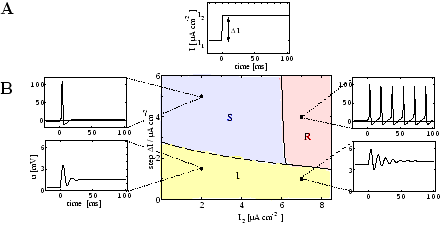
\includegraphics[width = 0.8\textwidth]{./pictures/gerstner.png}

    Step Current Stimulation Phase diagram
  \end{figure}
\end{frame}

\begin{frame}{Hypothesis}
  \begin{figure}
    \centering
    \[t = \frac{C_m}{I_m V_a}\] % time = capacitance over current times action potential
    \[f \propto J\] % frequency proportional to current density
    The train frequency is proportional to the current density
  \end{figure}
\end{frame}

\begin{frame}{Applications: Refractory Period}
  \begin{figure}
    \centering
    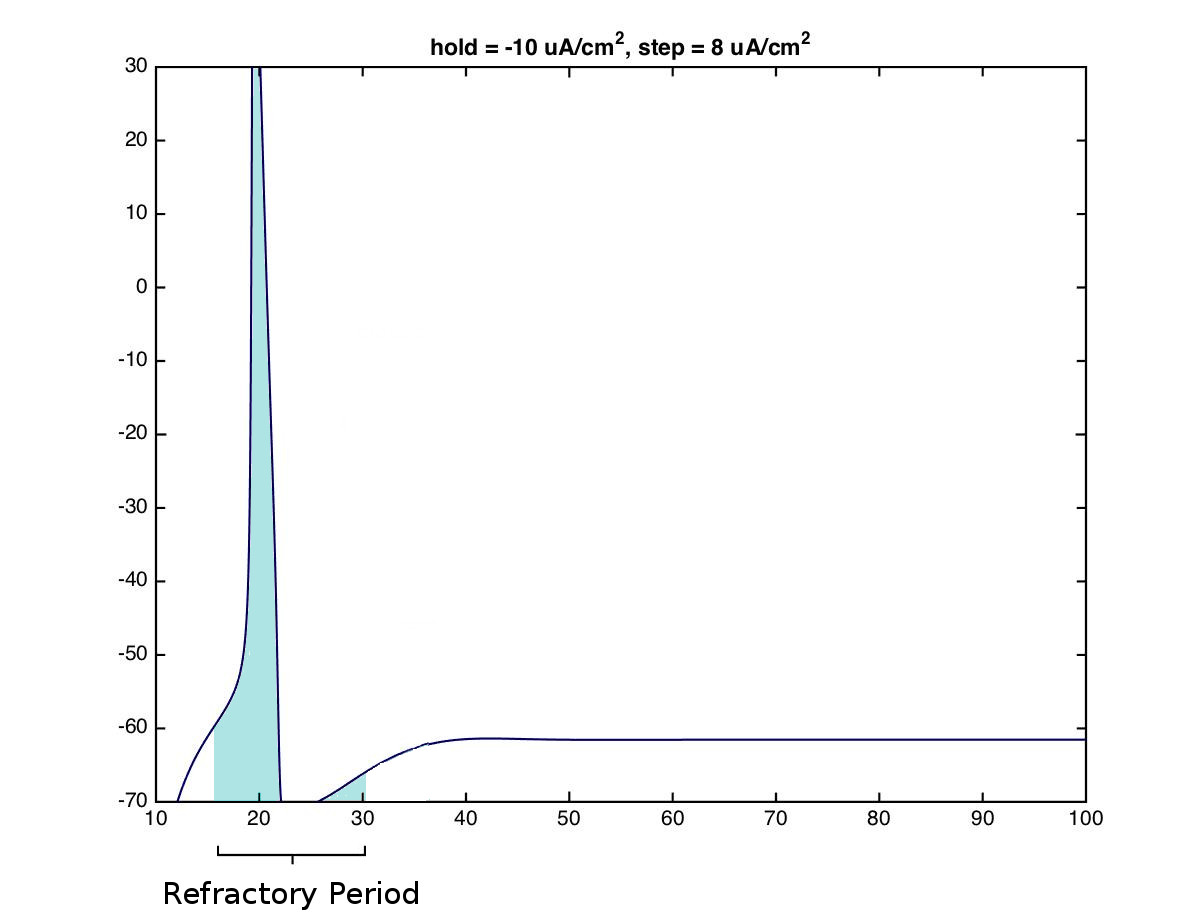
\includegraphics[width = 0.6\textwidth]{./pictures/refractory.jpg}
    \raisebox{0.4\height}{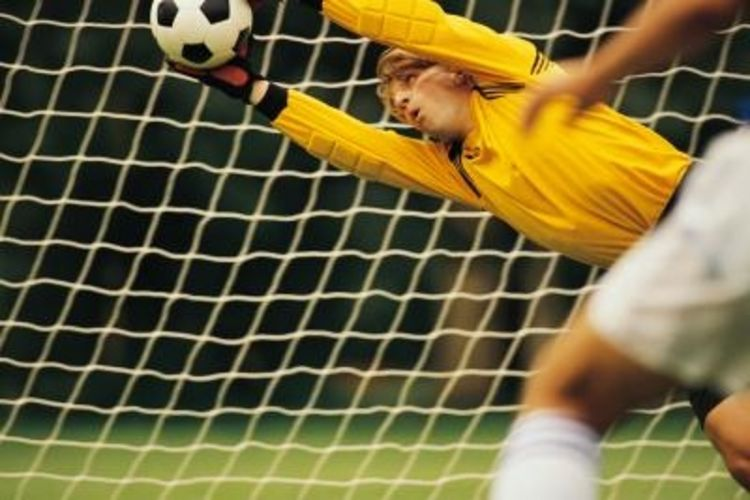
\includegraphics[width = 0.4\textwidth]{./pictures/reflexes.jpg}}

    Reducing the Refractory Period can lead to faster reflexes.
  \end{figure}
\end{frame}

\begin{frame}{Applications: Neuron Inhibition}
  \begin{figure}
    \centering
    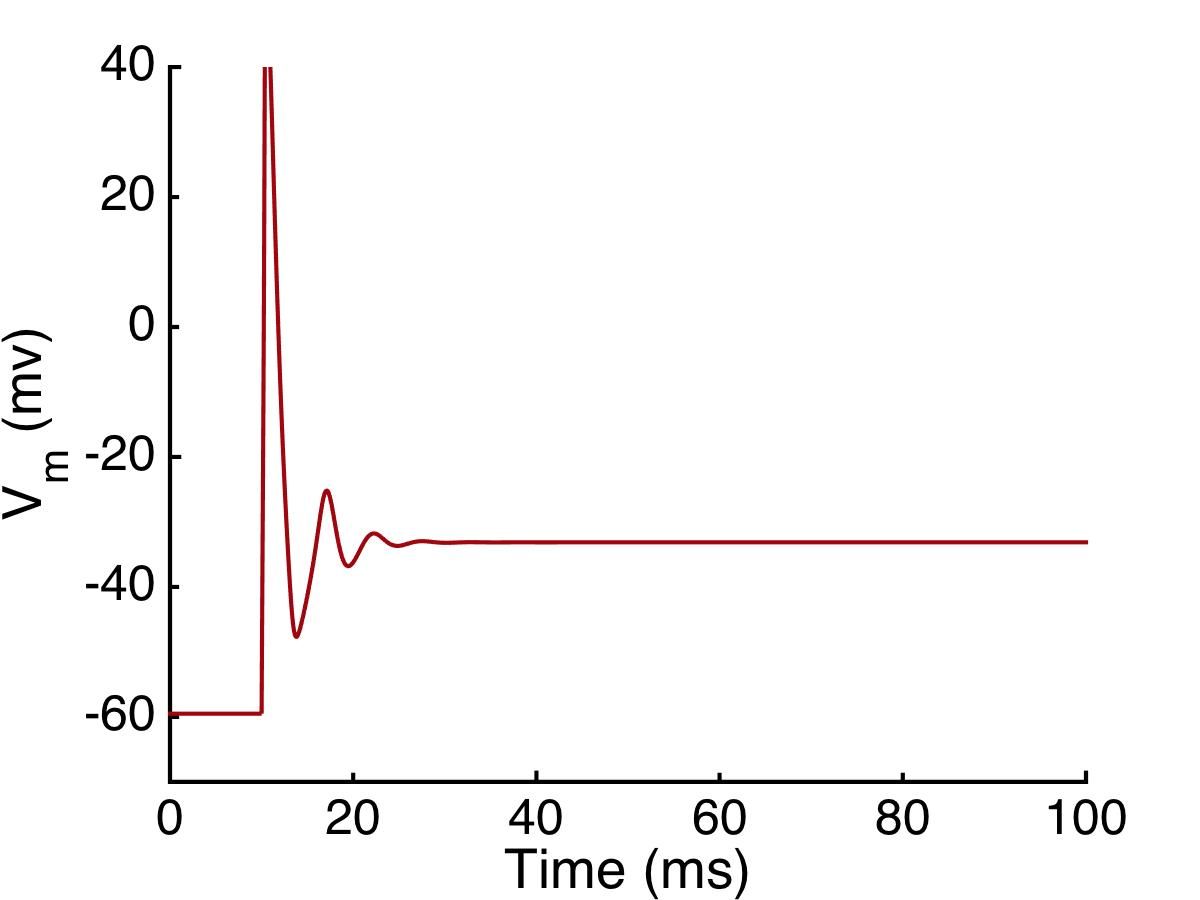
\includegraphics[width = 0.7\textwidth]{./images/current_0_250.jpg}

    High current fully damps neuron response
  \end{figure}
\end{frame}

\begin{frame}{Simulation Response Regions}
  \begin{figure}
    \centering
    \includegraphics[width = 0.33\textwidth]{./images/{current_0_2.4}.jpg}
    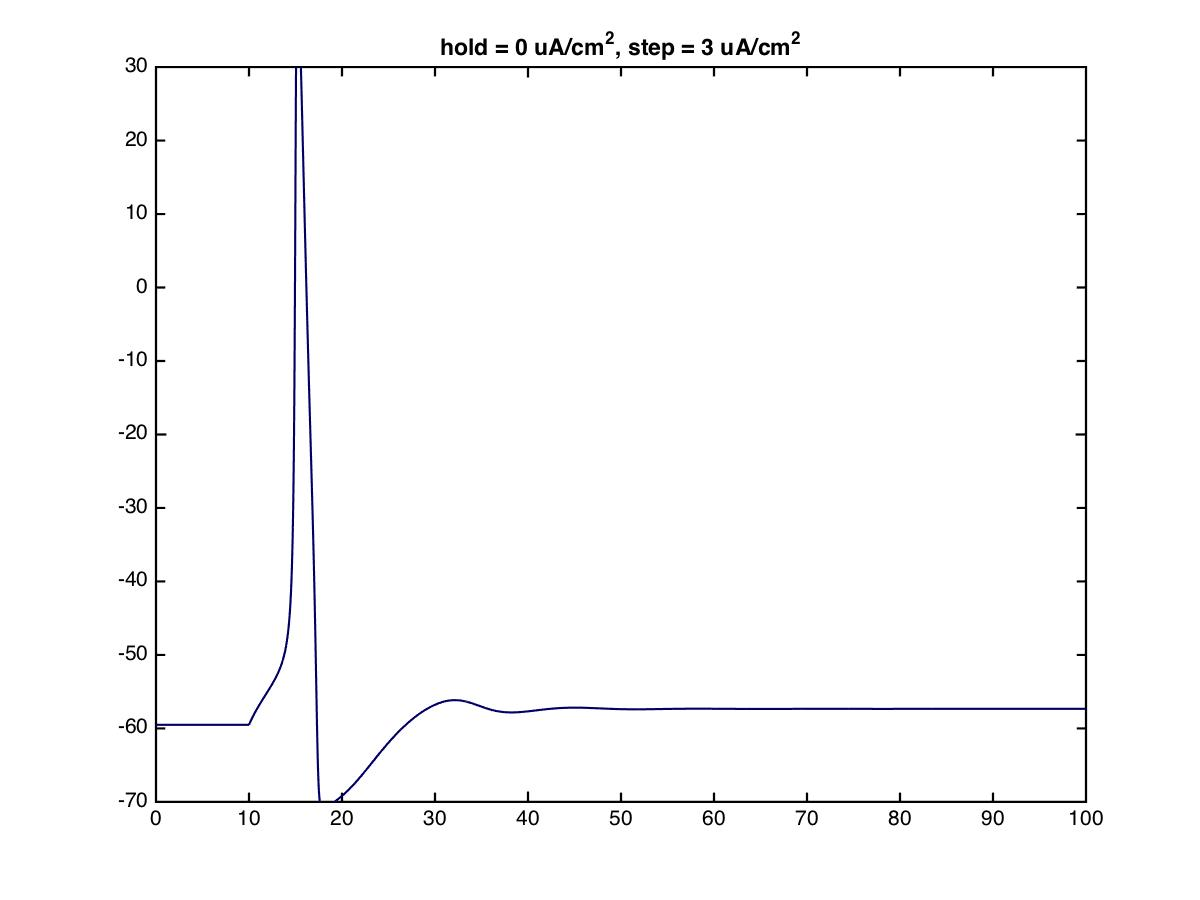
\includegraphics[width = 0.33\textwidth]{./images/current_0_3.jpg}
    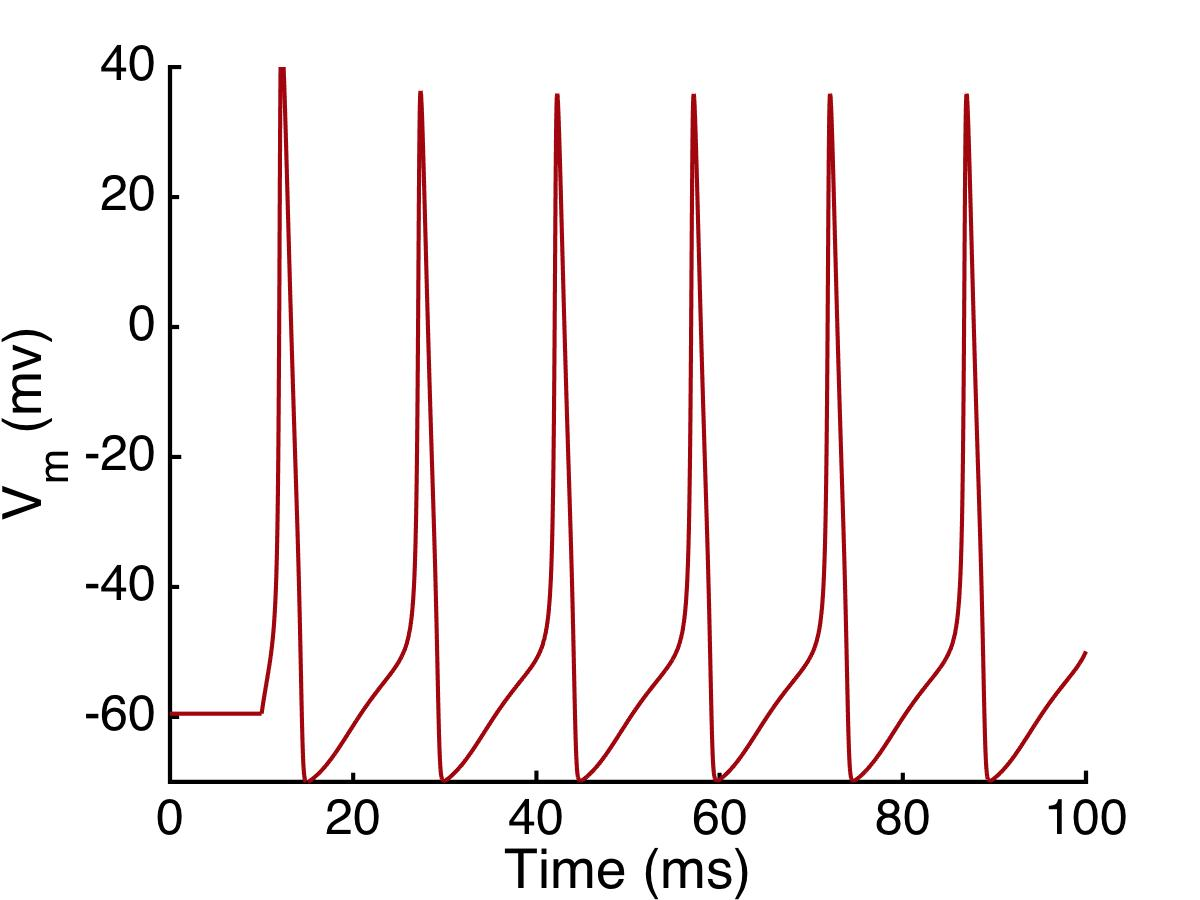
\includegraphics[width = 0.33\textwidth]{./images/current_0_10.jpg}

    Response in the \emph{Ringing}, \emph{Single AP} and \emph{AP Train} regions
  \end{figure}
\end{frame}

% slide 10
\begin{frame}{HH Model Action Train}
  \begin{figure}
    \centering
    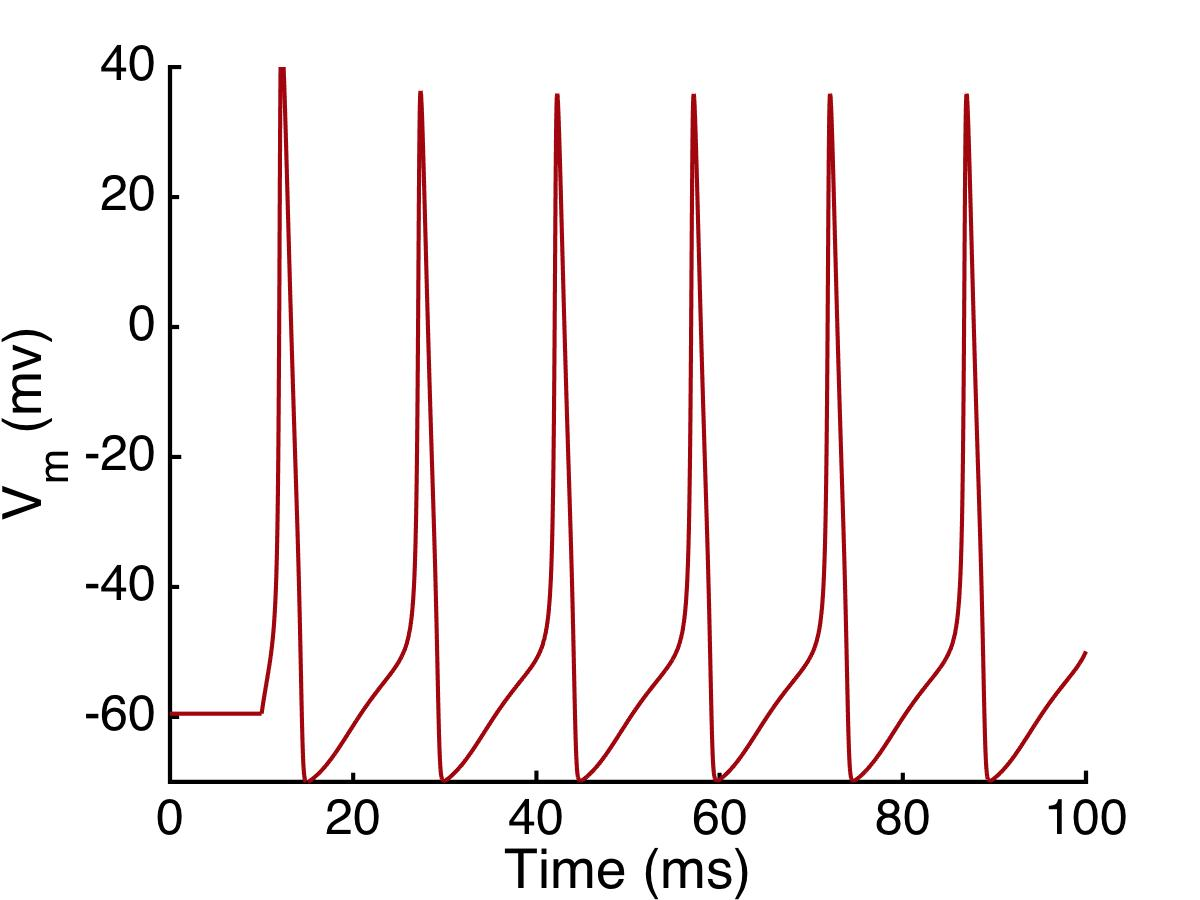
\includegraphics[width = 0.7\textwidth]{./images/current_0_10.jpg}

    Stepping to 10 $\mu A/cm^2$
  \end{figure}
\end{frame}


% slide 15
\begin{frame}{HH Model Action Train}
  \begin{figure}
    \centering
    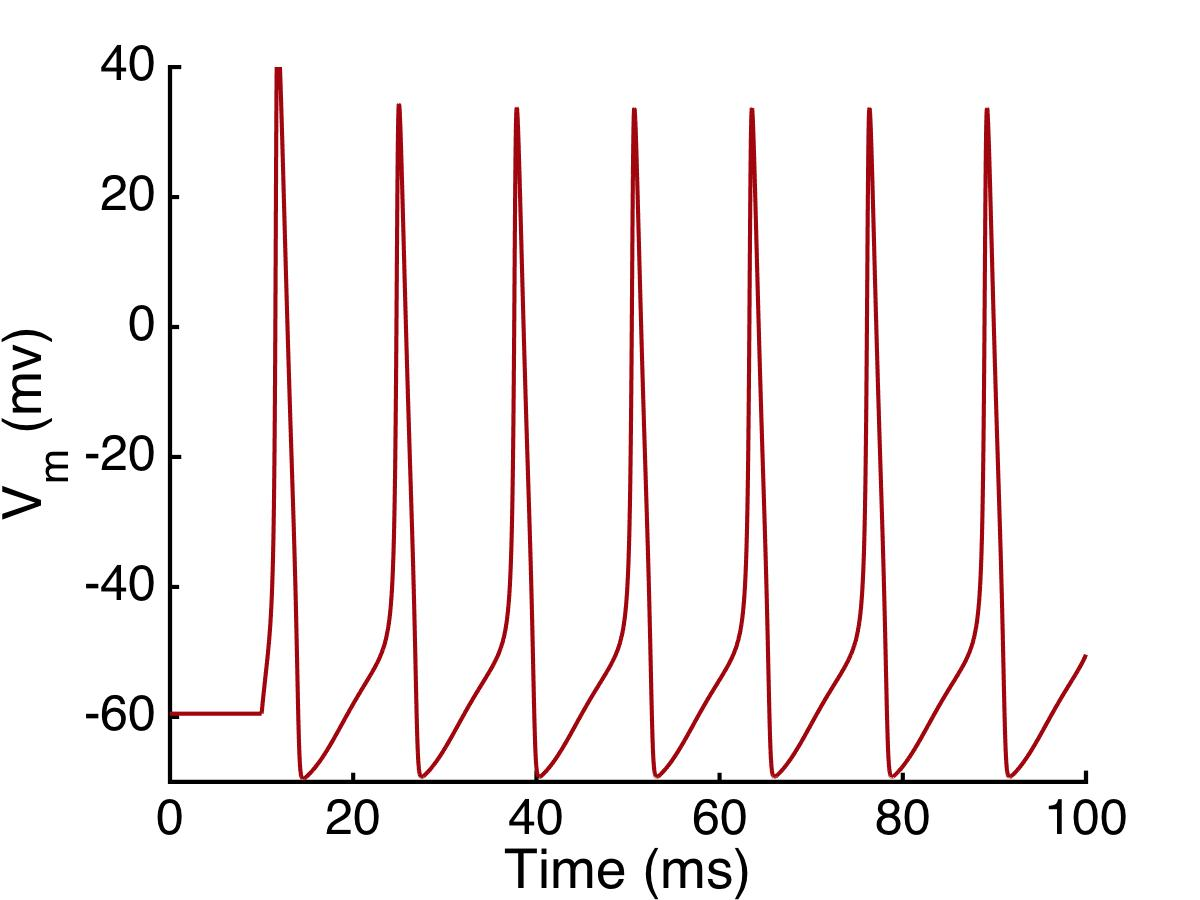
\includegraphics[width = 0.7\textwidth]{./images/current_0_15.jpg}

    Stepping to 15 $\mu A/cm^2$
  \end{figure}
\end{frame}


% slide 20
\begin{frame}{HH Model Action Train}
  \begin{figure}
    \centering
    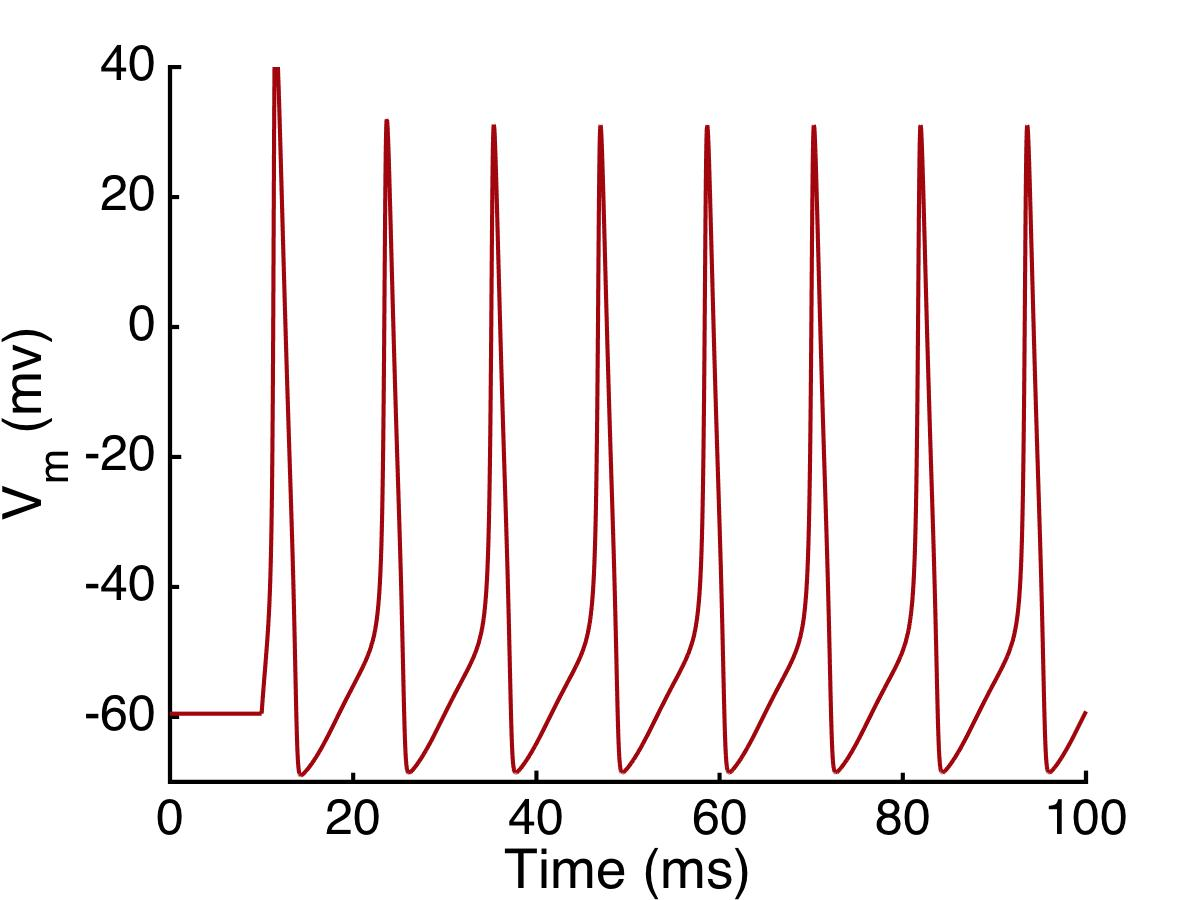
\includegraphics[width = 0.7\textwidth]{./images/current_0_20.jpg}

    Stepping to 20 $\mu A/cm^2$
  \end{figure}
\end{frame}


% slide 25
\begin{frame}{HH Model Action Train}
  \begin{figure}
    \centering
    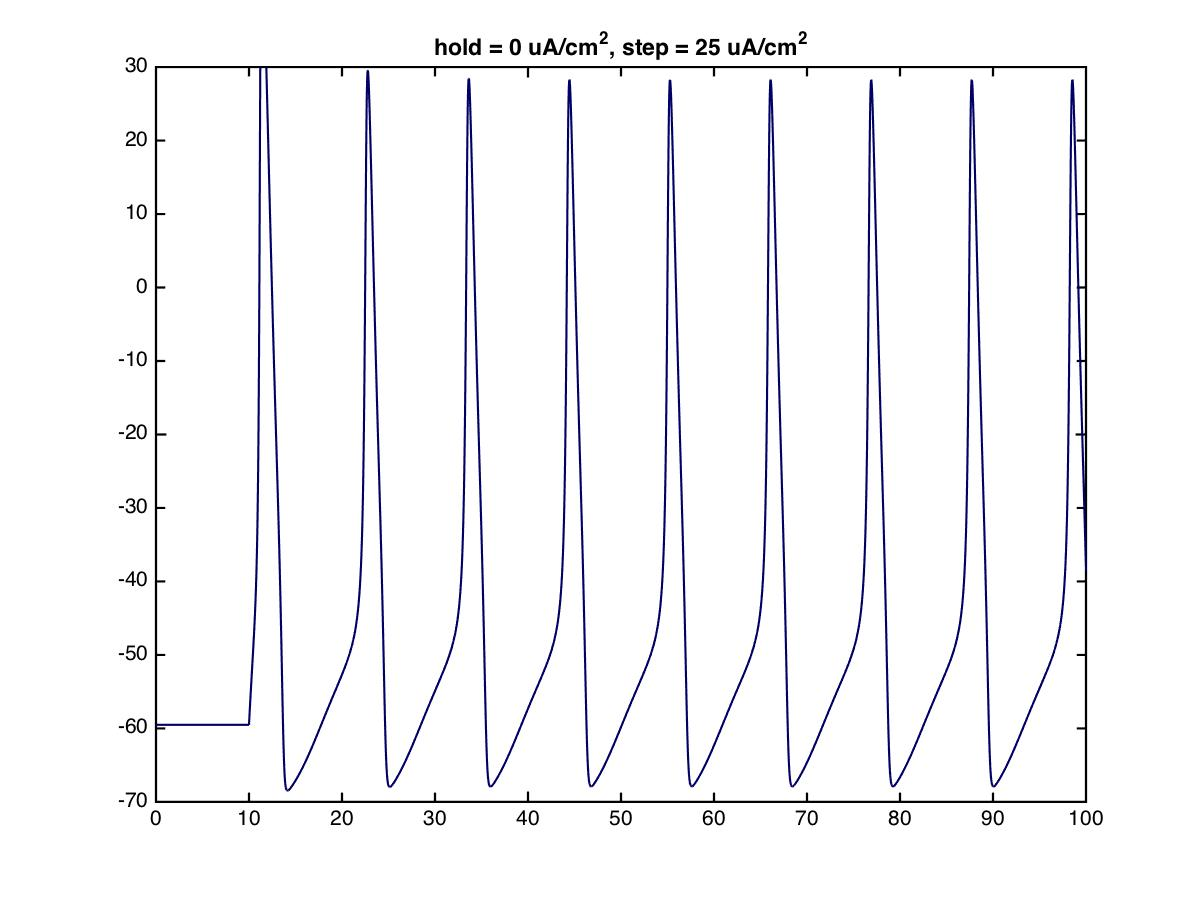
\includegraphics[width = 0.7\textwidth]{./images/current_0_25.jpg}

    Stepping to 25 $\mu A/cm^2$
  \end{figure}
\end{frame}


% slide 30
\begin{frame}{HH Model Action Train}
  \begin{figure}
    \centering
    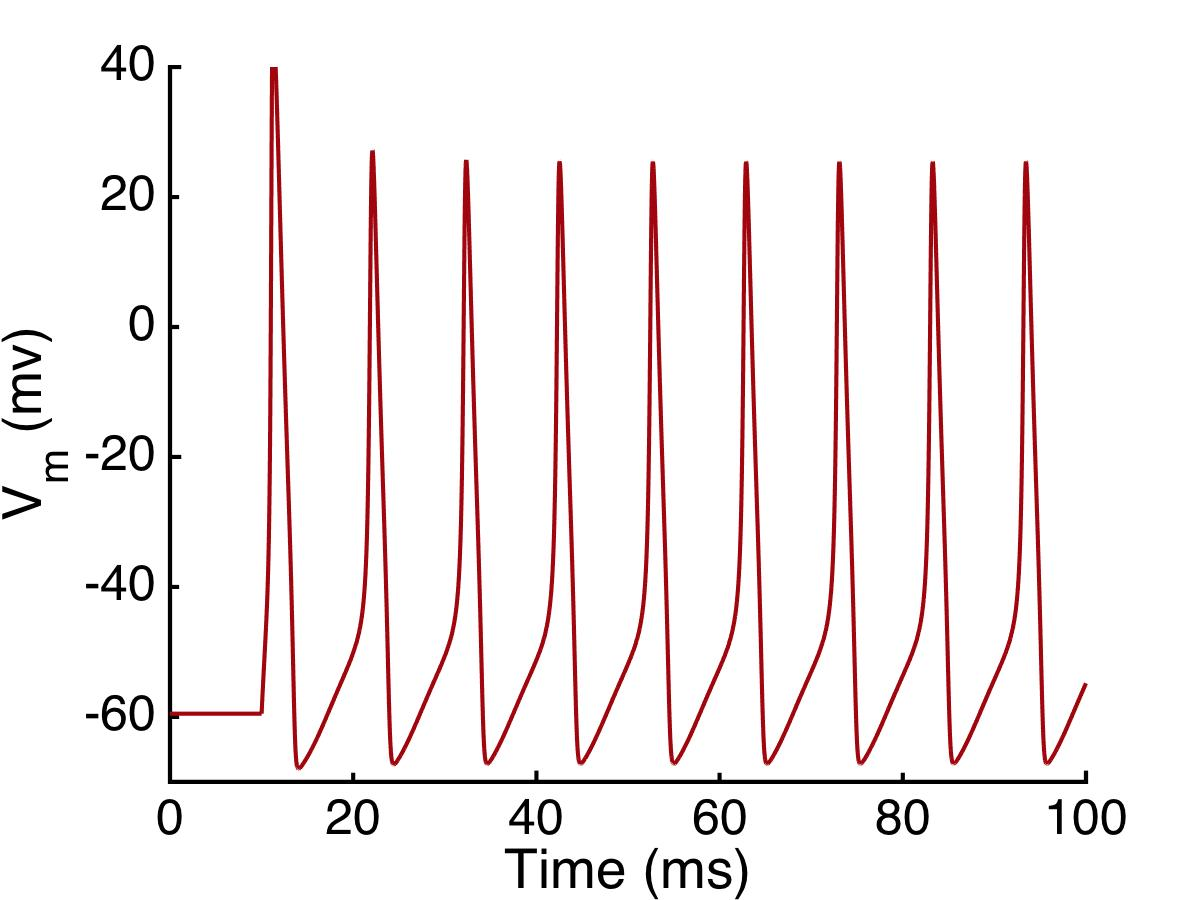
\includegraphics[width = 0.7\textwidth]{./images/current_0_30.jpg}

    Stepping to 30 $\mu A/cm^2$
  \end{figure}
\end{frame}


% slide 35
\begin{frame}{HH Model Action Train}
  \begin{figure}
    \centering
    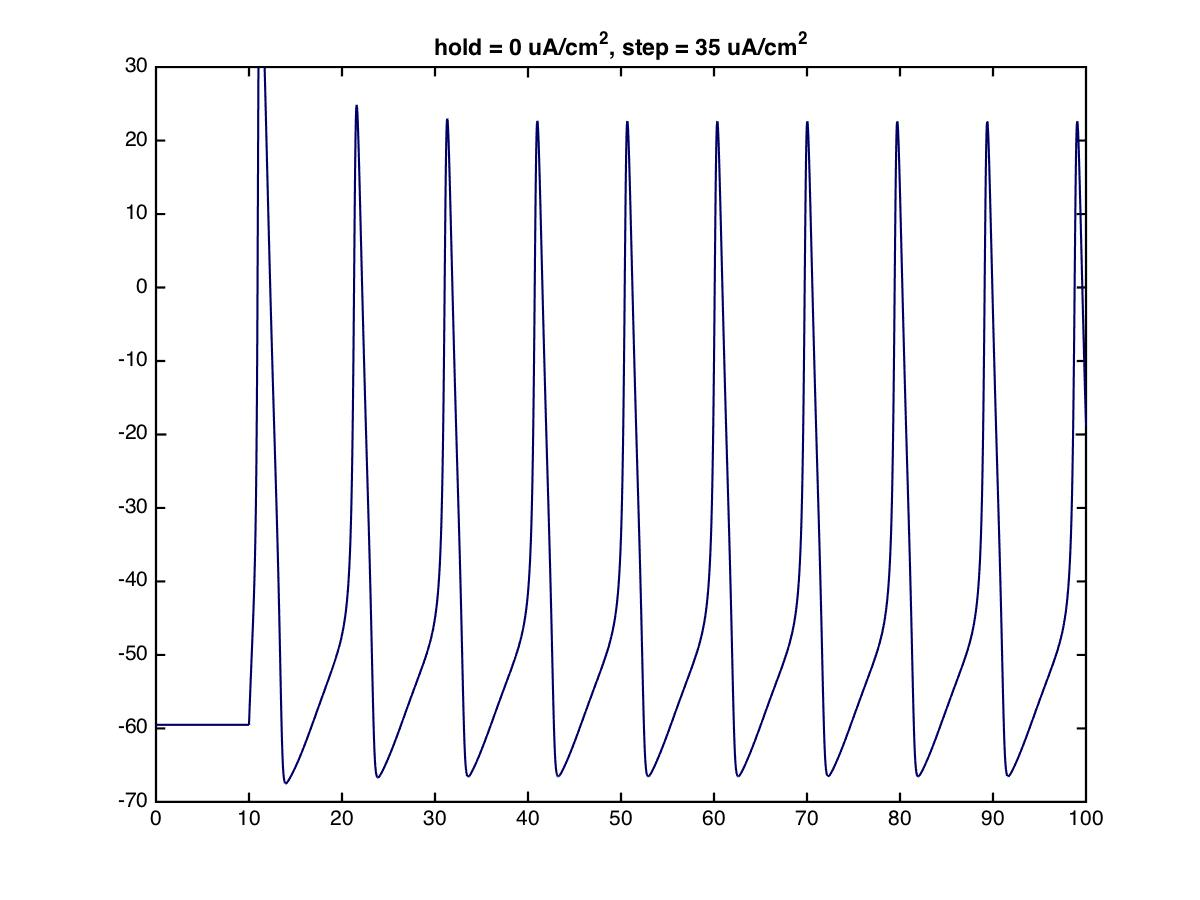
\includegraphics[width = 0.7\textwidth]{./images/current_0_35.jpg}

    Stepping to 35 $\mu A/cm^2$
  \end{figure}
\end{frame}

% slide 40
\begin{frame}{HH Model Action Train}
  \begin{figure}
    \centering
    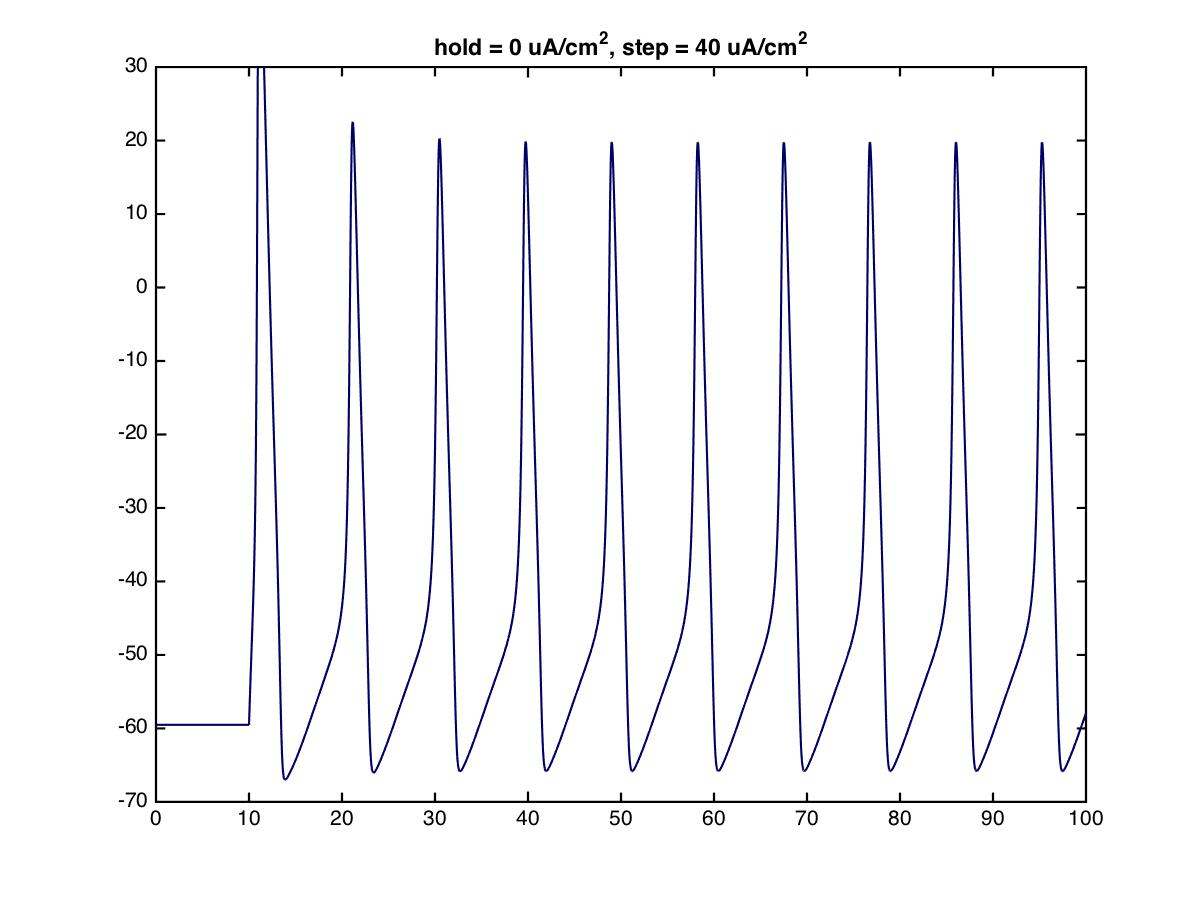
\includegraphics[width = 0.7\textwidth]{./images/current_0_40.jpg}

    Stepping to 40 $\mu A/cm^2$
  \end{figure}
\end{frame}


% slide 45
\begin{frame}{HH Model Action Train}
  \begin{figure}
    \centering
    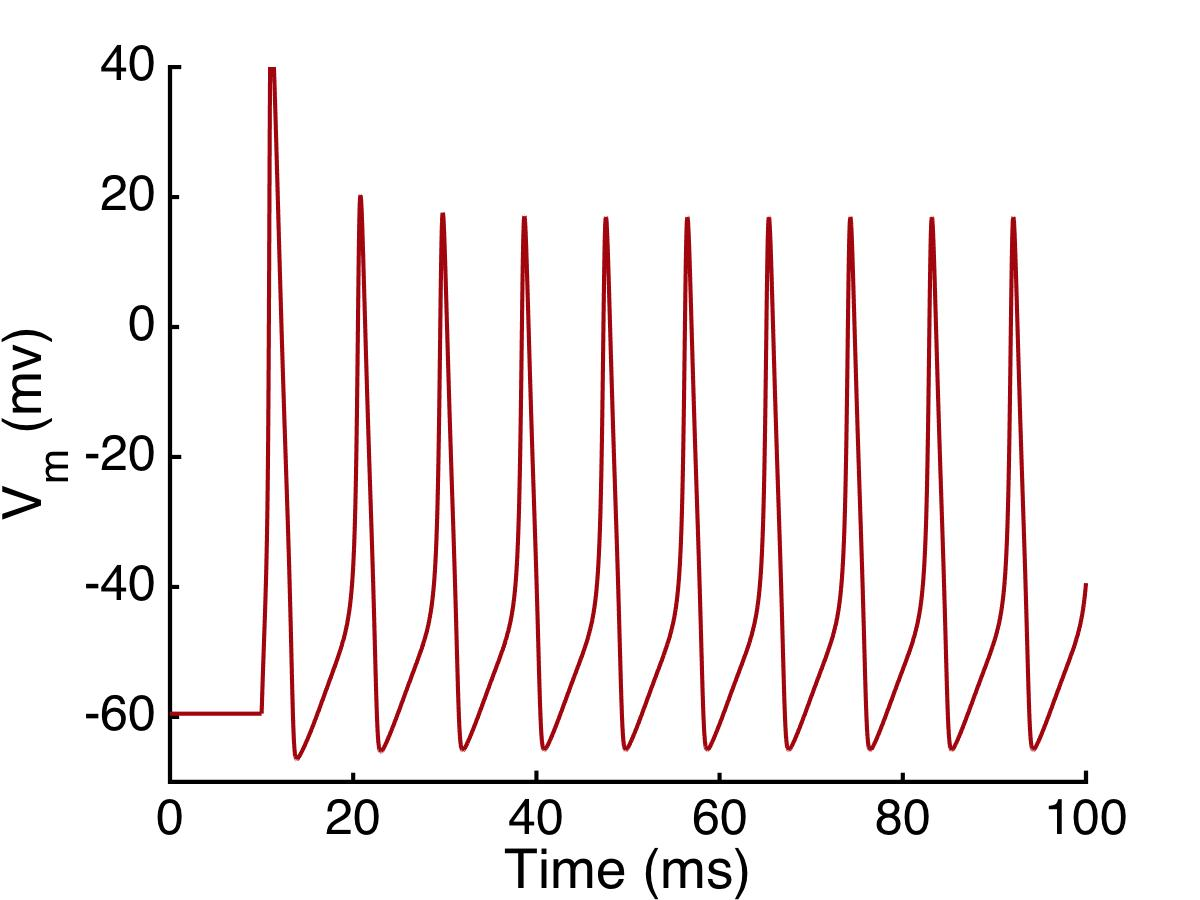
\includegraphics[width = 0.7\textwidth]{./images/current_0_45.jpg}

    Stepping to 45 $\mu A/cm^2$
  \end{figure}
\end{frame}


% slide 50
\begin{frame}{HH Model Action Train}
  \begin{figure}
    \centering
    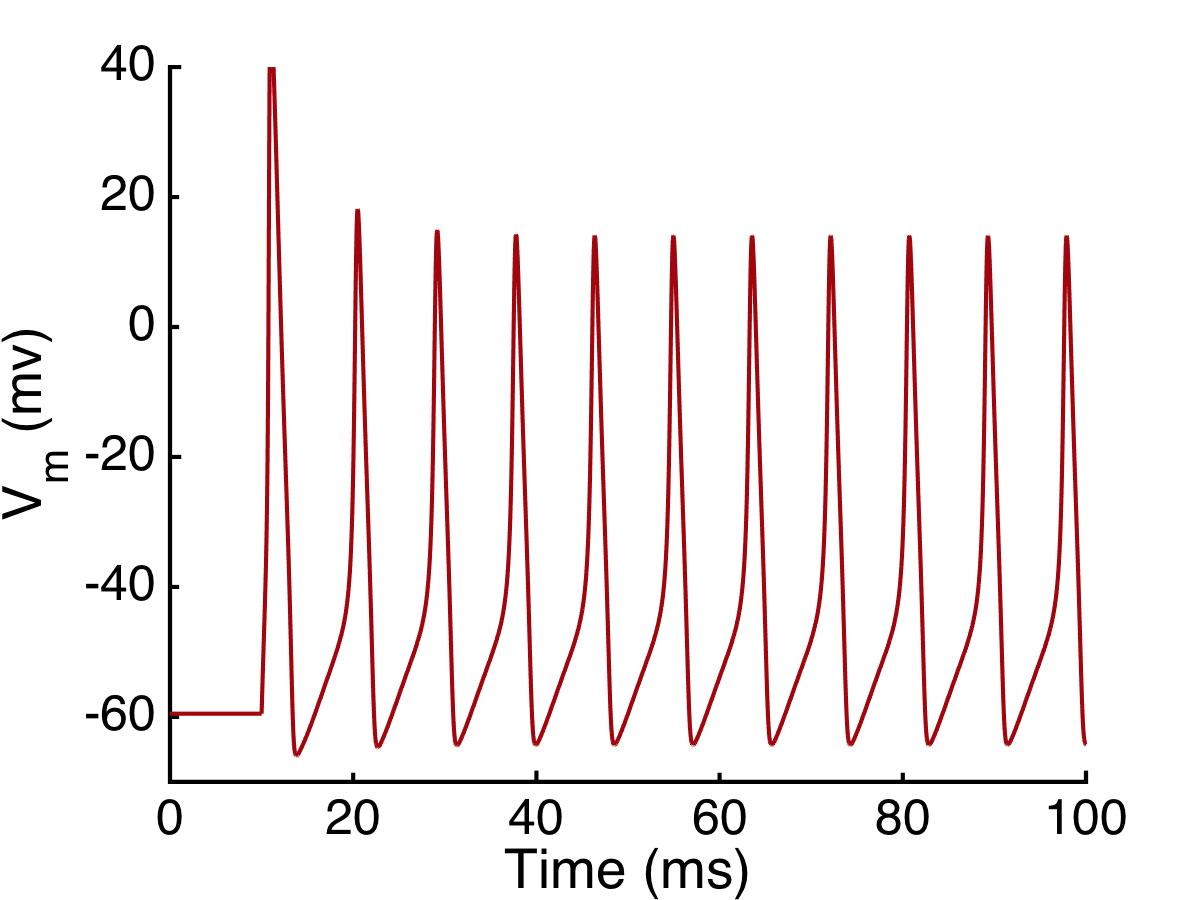
\includegraphics[width = 0.7\textwidth]{./images/current_0_50.jpg}

    Stepping to 50 $\mu A/cm^2$
  \end{figure}
\end{frame}


% slide 55
\begin{frame}{HH Model Action Train}
  \begin{figure}
    \centering
    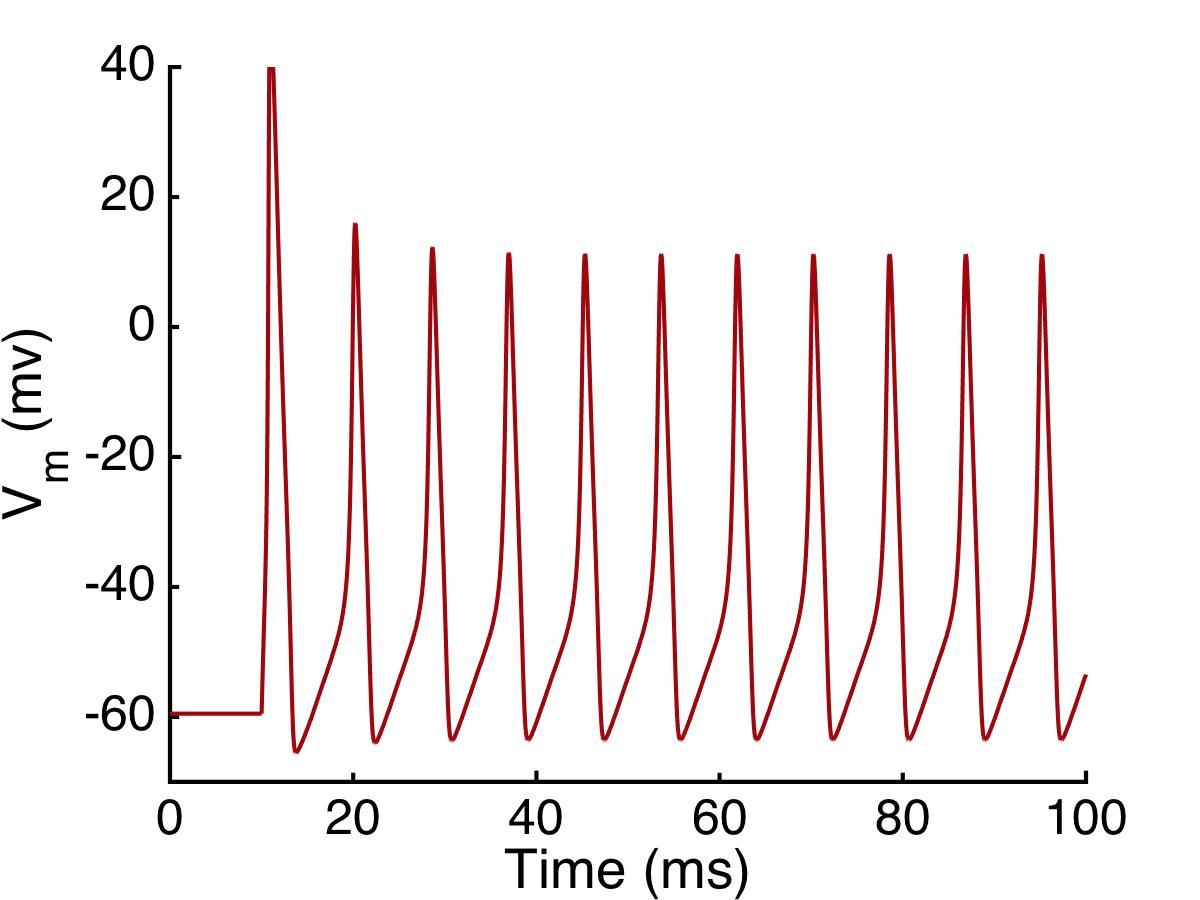
\includegraphics[width = 0.7\textwidth]{./images/current_0_55.jpg}

    Stepping to 55 $\mu A/cm^2$
  \end{figure}
\end{frame}


% slide 60
\begin{frame}{HH Model Action Train}
  \begin{figure}
    \centering
    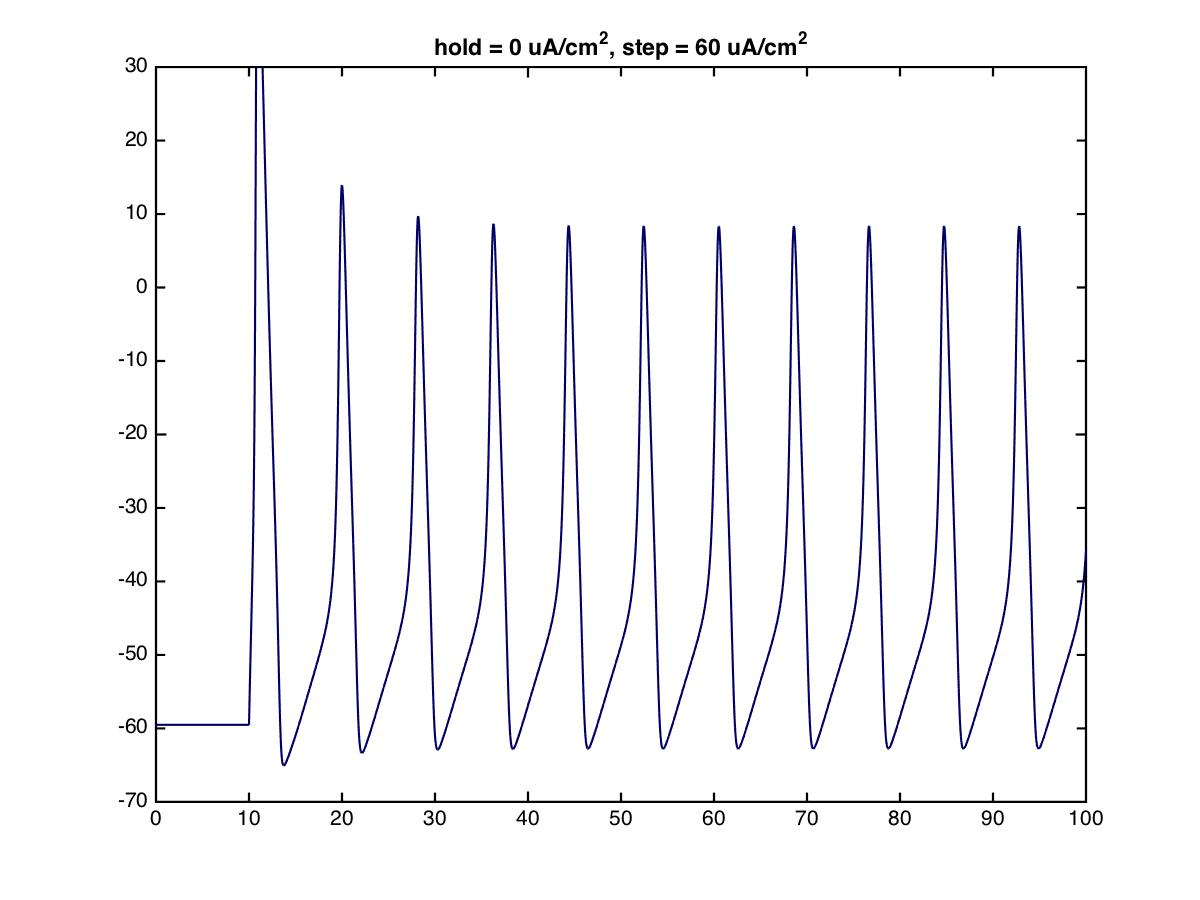
\includegraphics[width = 0.7\textwidth]{./images/current_0_60.jpg}

    Stepping to 60 $\mu A/cm^2$
  \end{figure}
\end{frame}


% slide 65
\begin{frame}{HH Model Action Train}
  \begin{figure}
    \centering
    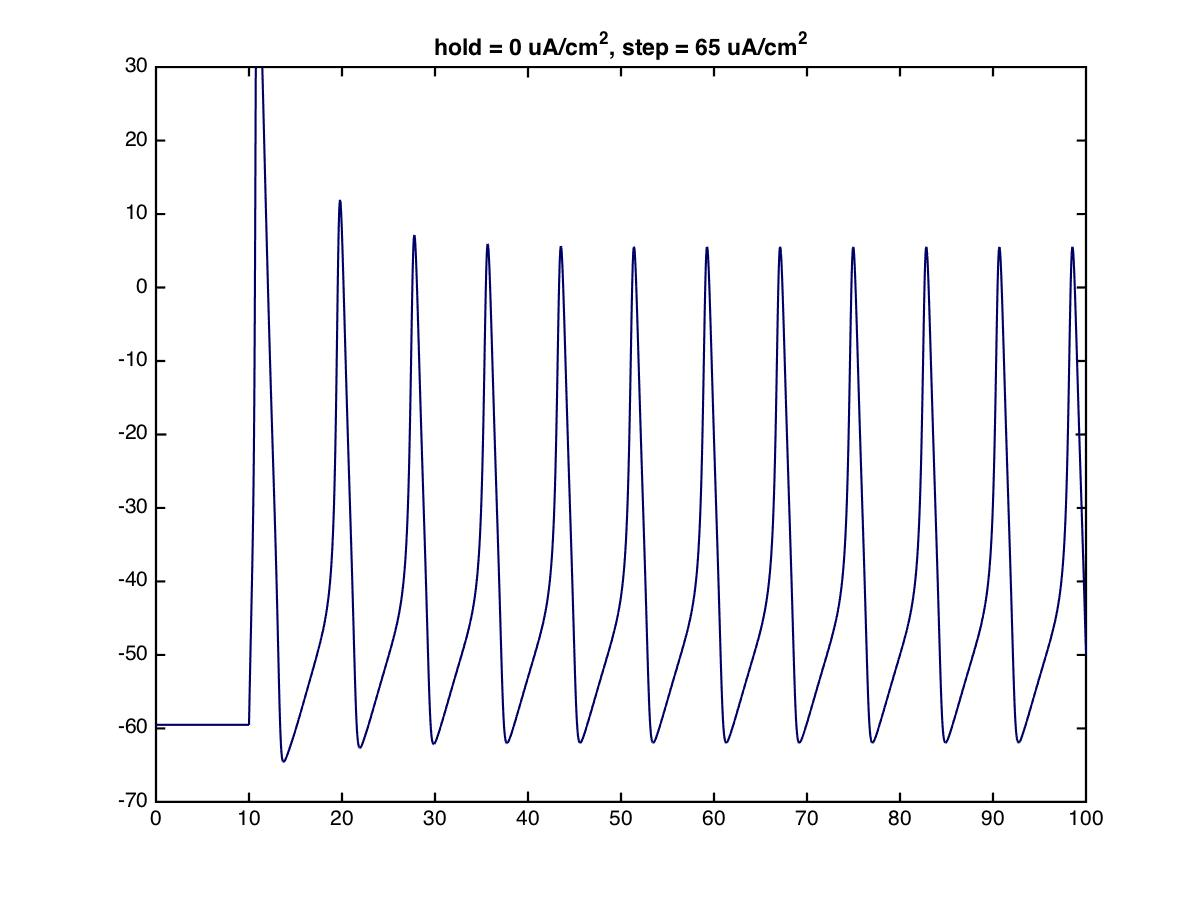
\includegraphics[width = 0.7\textwidth]{./images/current_0_65.jpg}

    Stepping to 65 $\mu A/cm^2$
  \end{figure}
\end{frame}


% slide 70
\begin{frame}{HH Model Action Train}
  \begin{figure}
    \centering
    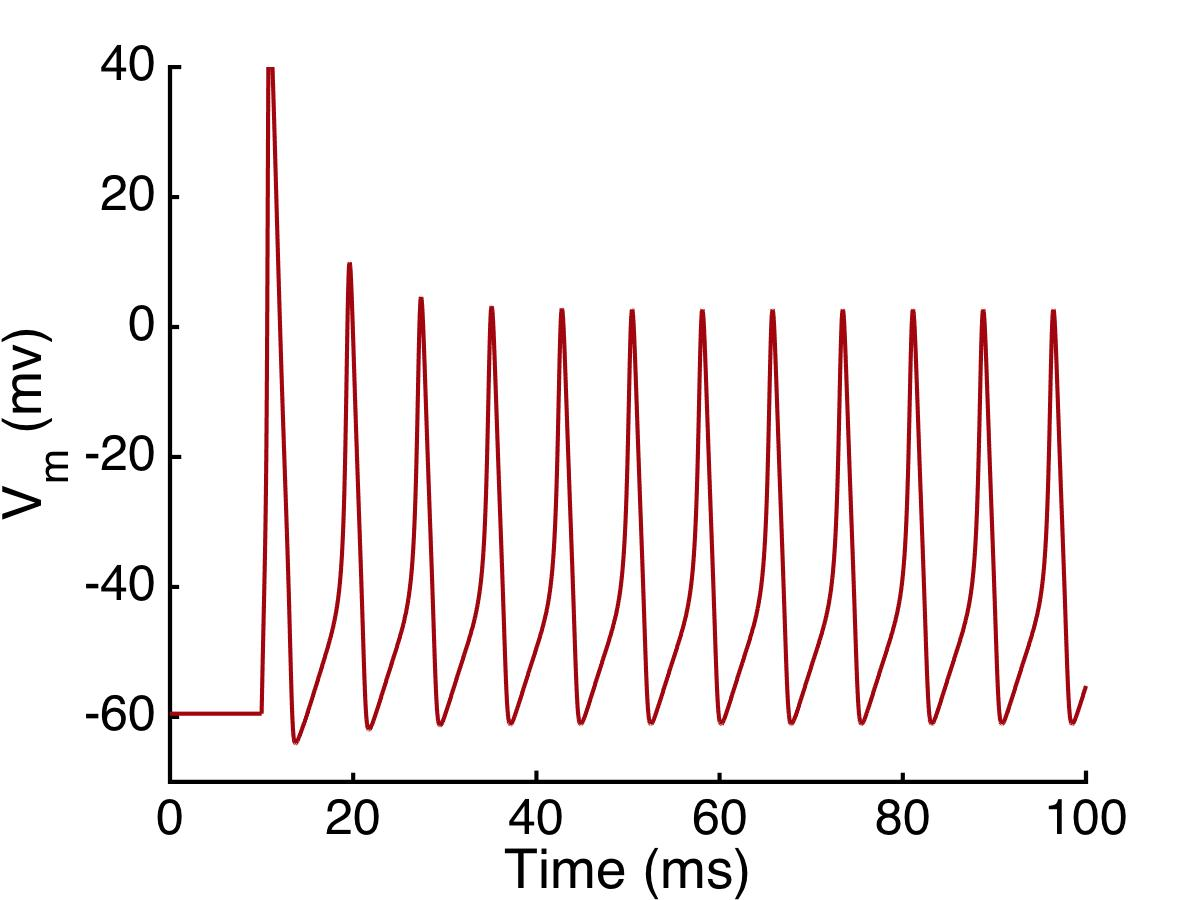
\includegraphics[width = 0.7\textwidth]{./images/current_0_70.jpg}

    Stepping to 70 $\mu A/cm^2$
  \end{figure}
\end{frame}


% slide 75
\begin{frame}{HH Model Action Train}
  \begin{figure}
    \centering
    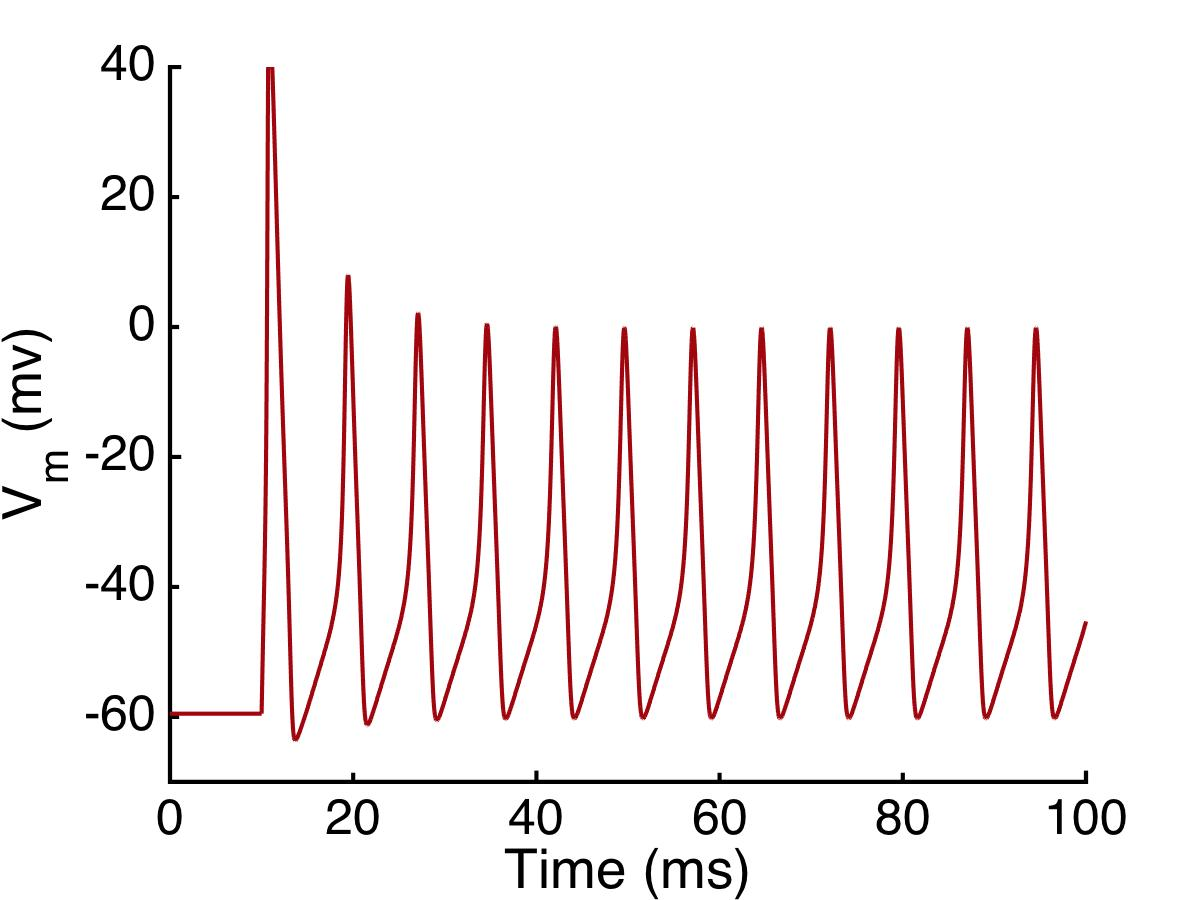
\includegraphics[width = 0.7\textwidth]{./images/current_0_75.jpg}

    Stepping to 75 $\mu A/cm^2$
  \end{figure}
\end{frame}


% slide 80
\begin{frame}{HH Model Action Train}
  \begin{figure}
    \centering
    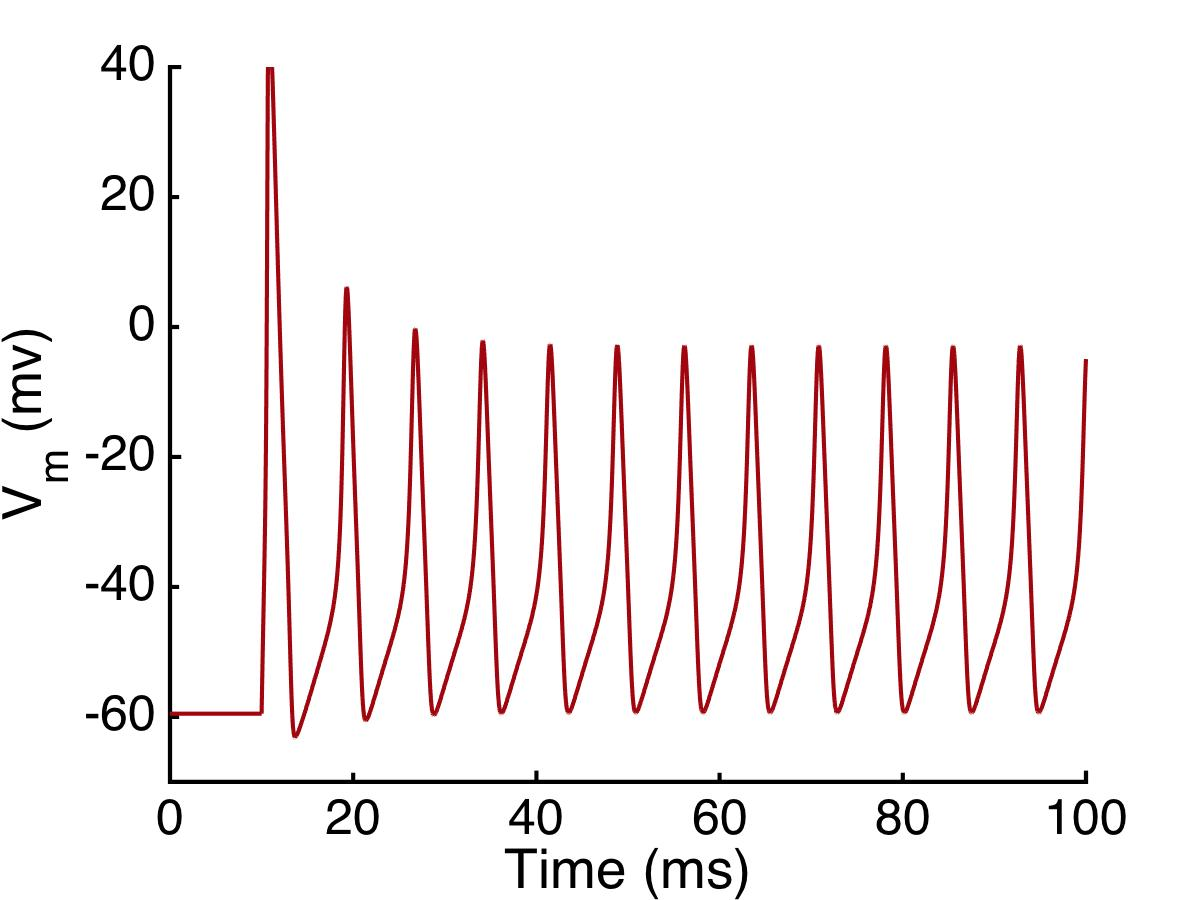
\includegraphics[width = 0.7\textwidth]{./images/current_0_80.jpg}

    Stepping to 80 $\mu A/cm^2$
  \end{figure}
\end{frame}

\begin{frame}{Fourier Transform Insufficient: Inconsistent Time Intervals}
  \begin{figure}
    \centering
    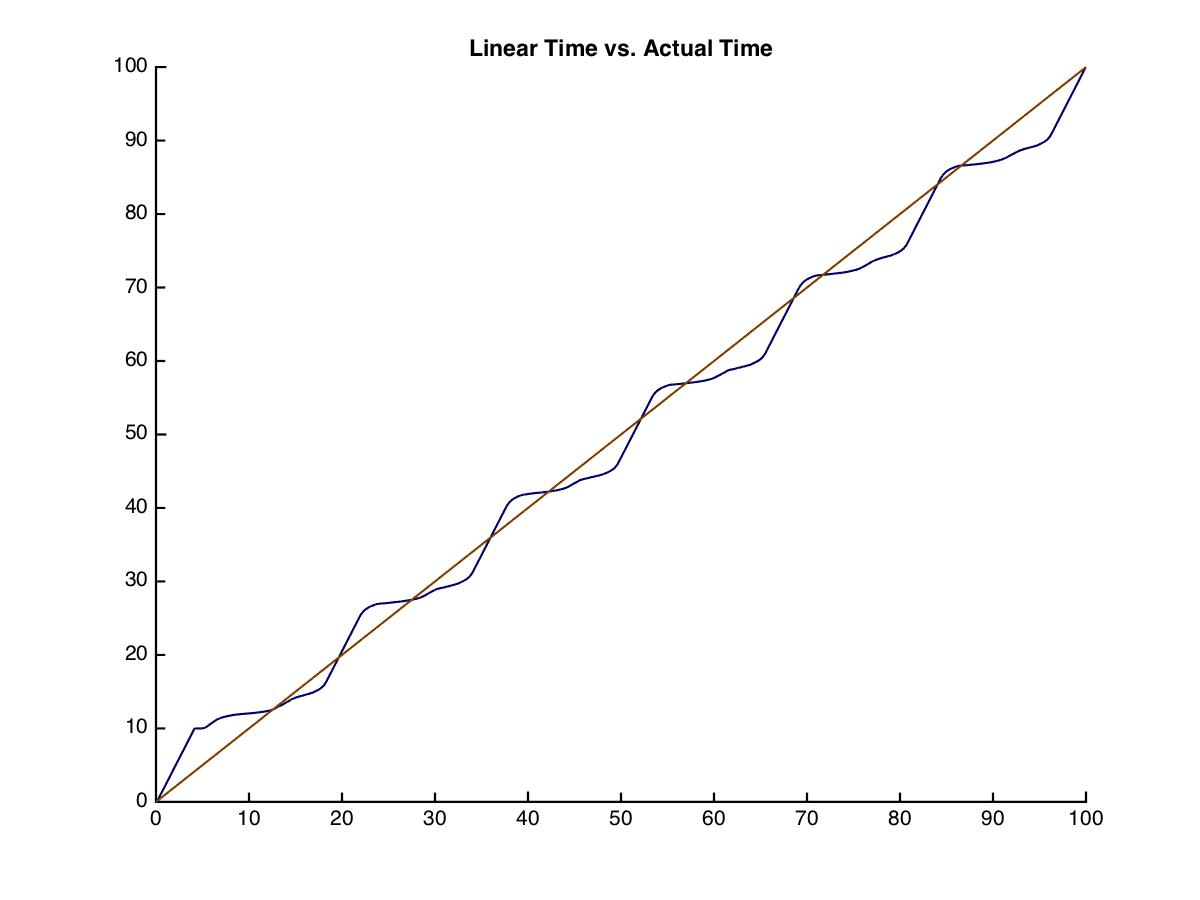
\includegraphics[width = 0.7\textwidth]{./images/lintimevsactualtime.jpg}

    FFT insufficient, need a better Spectral Analysis Method
  \end{figure}
\end{frame}

\begin{frame}{Least-Squares Spectral Analysis}
  \begin{figure}
    \centering
    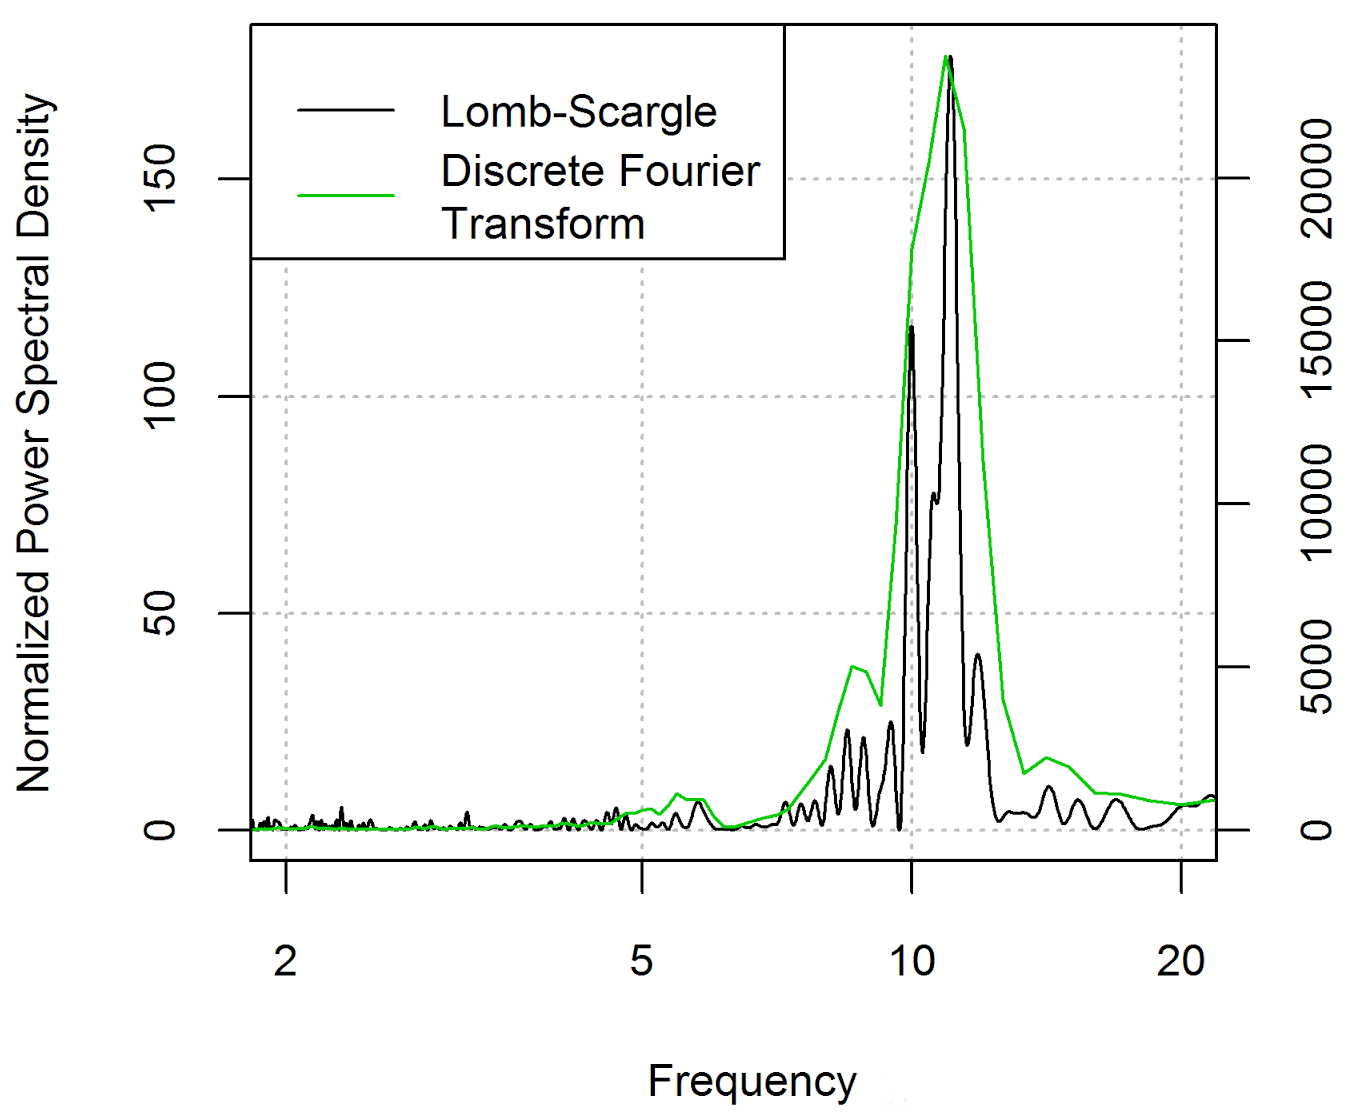
\includegraphics[width = 0.6\textwidth]{./pictures/lomb_vs_FFT.png}

    The Lomb-Scargle Periodogram works with variable intervals.
  \end{figure}
\end{frame}

\begin{frame}{Graphing the Train Frequency}
  \begin{figure}
    \centering
    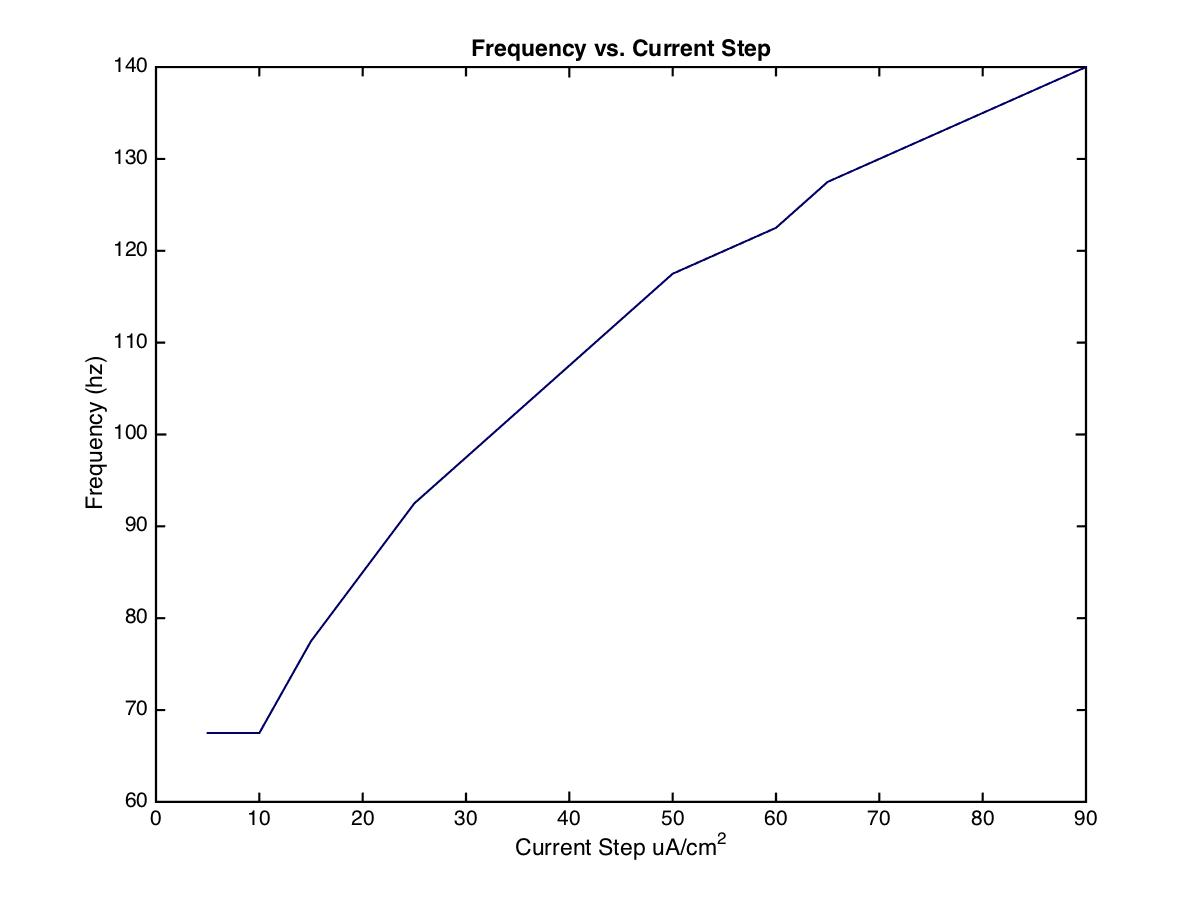
\includegraphics[width = 0.7\textwidth]{./images/freqvscurrent.jpg}

    Nonlinearity shows complexity of behavior
  \end{figure}
\end{frame}

\begin{frame}{Naive Mechanism}
  \begin{figure}
    \centering
    \includegraphics[width = 0.7\textwidth]{./images/{cap_1.5vs1.5}.jpg}

    Equal ratio of current to capacitance
  \end{figure}
\end{frame}

\begin{frame}{Mechanism}
  \begin{figure}
    \centering
    \includegraphics[width = 0.7\textwidth]{./images/{cap_1.5vs2.4}.jpg}

    Unequal ratio of current to capacitance
  \end{figure}
\end{frame}


\begin{frame}{Conclusion}
  \begin{enumerate}
    \item Innovative experimental method
    \item Clear definition of saturation threshold
    \item High accuracy prediction of cell response
    \item Refuted possible simplification
  \end{enumerate}
\end{frame}

\begin{frame}{References}
\begin{enumerate}
\item Weiss, T. F. (1995).Cellular Biophysics. Volume 1: Transport, MIT Press.
\item Weiss, T. F. (1995).Cellular Biophysics. Volume 2: Electrical Properties, MIT Press.
\item Blaustein, M.P., Kao, J.P.Y., Matteson, D.R. (2012). Cellular Physiology and Neurophysiology, 2nd edition, Elsevier-Mosby.
\item Gerstner, Wulfram, and Werner M. Kistler. Spiking neuron models: Single neurons, populations, plasticity. Cambridge university press, 2002.
\item Press, William H., and George B. Rybicki. ``Fast algorithm for spectral analysis of unevenly sampled data.'' The Astrophysical Journal 338 (1989): 277--280.
\end{enumerate}
\end{frame}

\begin{frame}{Anomalies With Default HH Model Settings}
  \begin{figure}
    \centering
    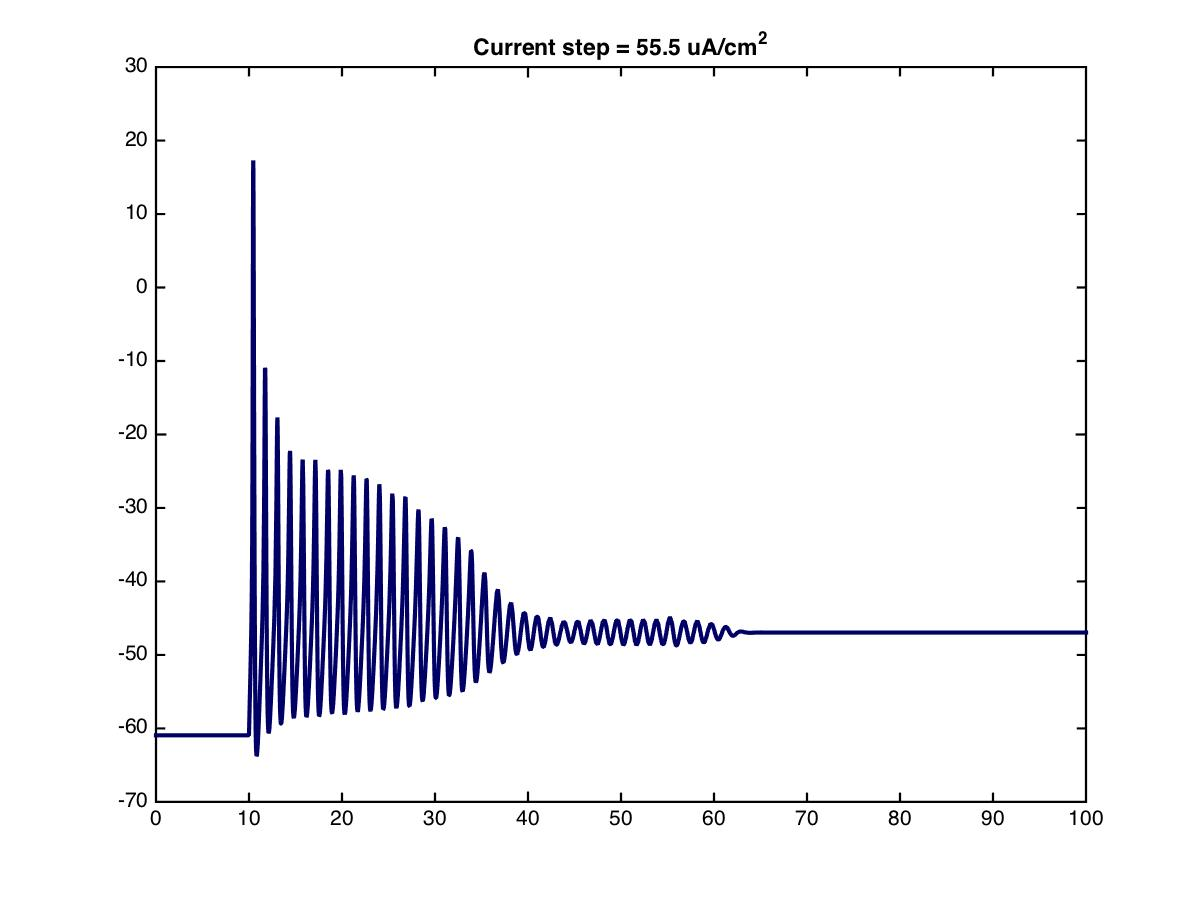
\includegraphics[width = 0.4\textwidth]{./images/current55p5.jpg}
    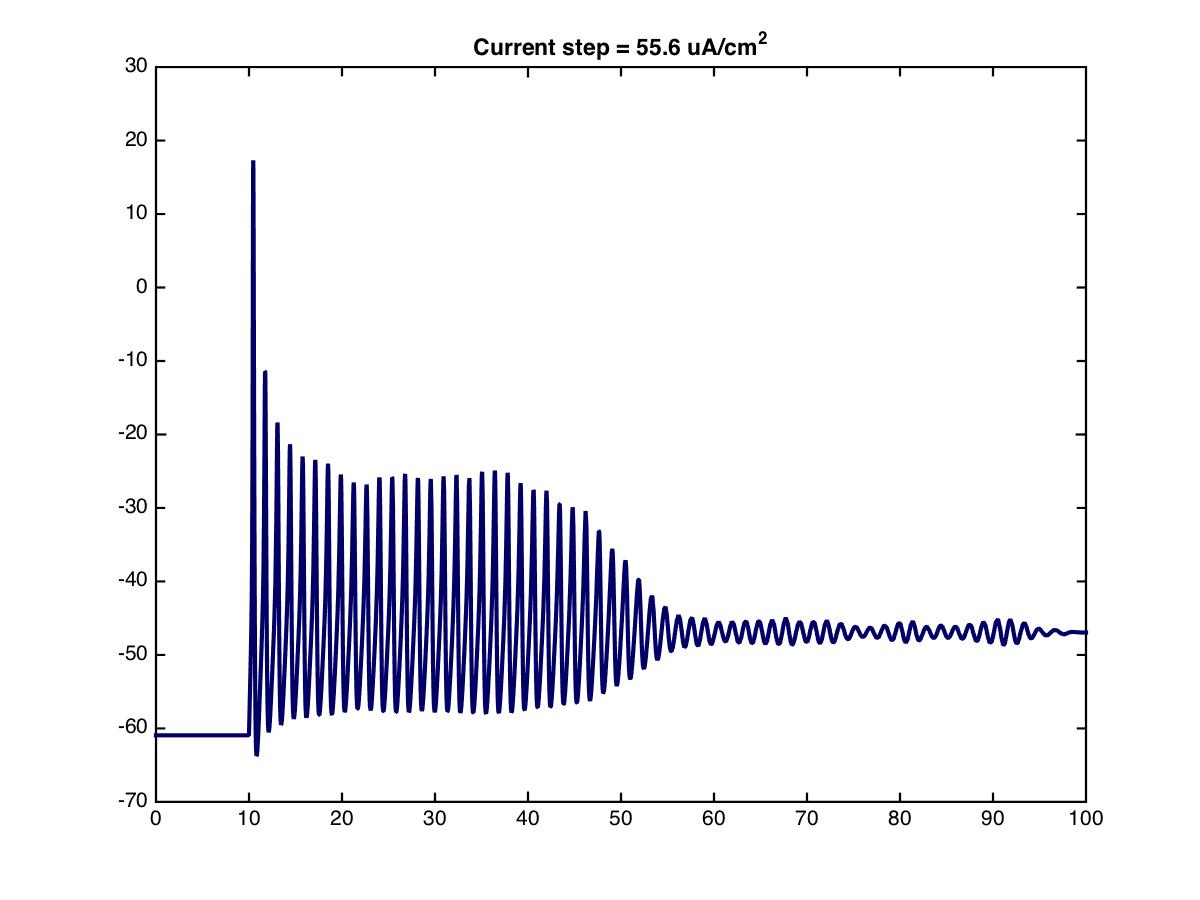
\includegraphics[width = 0.4\textwidth]{./images/current55p6.jpg}

    Incorrect behavior due to low precision
  \end{figure}
\end{frame}

\end{document}
